\documentclass[a4paper,12pt]{article}
\usepackage[utf8]{inputenc}
\usepackage{graphicx}
\usepackage{multicolumn}
\usepackage{multirow}
\usepackage{booktabs}
\usepackage[indent=0pt,skip=3mm]{parskip}
\usepackage{array}
\usepackage{commath} % for abs ||
\usepackage{listings}             % Include the listings-package
\usepackage{tabs}
% \usepackage{colortbl}
\usepackage{url}
\usepackage{datetime}
\usepackage[ top=5cm, left=1.5cm, right=1.5cm, headheight=4cm,bottom=1cm]{geometry}
\usepackage{lastpage} % include last page numbering
\usepackage{fancyhdr}
\usepackage[table]{xcolor}% ctan.org/pkg/xcolor %FOR COLORS
% \usepackage{frame}
\settimeformat{xxivtime}
\setdefaultdate{\ddmmyyyydate}
\hyphenation{matriz}
\graphicspath{{figures/}{./images/}}
\newcommand{\eq}[1]{$#1$}
\newcommand{\head}[1]{{\bfseries #1}}
\newcommand{\header}[2][\tiny]{{\bfseries #1 #2}}

%%%%%%%%%%%%%%%%%%%%%%%%%%%%%%%%%%%%%%%%%%%%%%%%%%%%%%%%%%%%%%%%%%%%%%
%%%%%%%%%%%%%%%%%%%%%%%%%%%%%%%%%%%%%%%%%
\newsavebox{\mytabularheader}
\newsavebox{\mytabularheadertitle}
\setlength{\extrarowheight}{0.1cm}
%----------------------------------------------------------------------------------
%-----------------------------------------------------------------------------------------------
\sbox{\mytabularheadertitle}{%
  \begin{minipage}{.52\textwidth}
    \begin{center}
        \bfseries \scriptsize  UNIVERSIDAD NACIONAL DE SAN AGUSTIN\\
        FACULTAD DE INGENIERÍA DE PRODUCCIÓN Y SERVICIOS\\
        ESCUELA PROFESIONAL DE INGENIERÍA DE SISTEMA\\[3mm]
    \end{center}
  \end{minipage}
}

\sbox{\mytabularheader}{%
    \begin{minipage}{\textwidth}
        \centering
        \begin{tabular}{cp{8cm}c}
            
\includegraphics[scale=0.3]{epis_logo.png} & 
            \usebox{\mytabularheadertitle} &
            
\includegraphics[scale=0.05]{abet_logo.png} \\
            % \hline
            \multicolumn{3}{c}{Formato: Guía de Práctica de Laboratorio / Talleres / Centros de Simulación}\\
             &\multicolumn{1}{c}{Aprobación:  2022/03/01 Código: GUIA-PRLE-001} &  \\
        \end{tabular}
    \end{minipage}
}
%---------------------------------------
\renewcommand{\headrulewidth}{0pt}
\fancypagestyle{plain}{%
  \fancyhf{}%
  \fancyhf[ch]{\usebox{\mytabularheader}}
}
%--------------------------------------
\pagestyle{plain}
%%%%%%%%%%%%%%%%%%%%%%%%%%%%%%%%%%%%%%%%%%%%%%%%%%%%%%%%%%%%%%%%%%%%%%%%%%%%%%%%%%%%%%%%%%
\definecolor{blackRed}{cmyk}{0,81,76,31}

\begin{document}    
\lstset{language=Python,frame=single, firstnumber=1,basicstyle=\footnotesize,
numbers=left,showspaces=false,showstringspaces=false}   
    \begin{table}[t]
        \centering
        \begin{tabular}{|p{2.3cm}<{:}|m{1.7cm}|m{2.4cm}|m{2cm}|m{3cm}|m{0.6cm}|}
            \multicolumn{6}{c}{\cellcolor{red}{\leavevmode\color{white}\header{INFORMACIÓN BÁSICA}}}\\
            \hline
            \header{ASIGNATURA} & \multicolumn{5}{c}{\header[\footnotesize]{Física Computacional.}}\\
            \hline
            \header{\mbox{TÍTULO DE LA} PRÁCTICA} & \multicolumn{5}{c}{\header[\footnotesize]{Práctica de Ecuación diferencial de Laplace.}}\\
            \hline
            \header{\mbox{NÚMERO DE} PRÁCTICA} & {\header[\footnotesize]{05}} & \header{AÑO LECTIVO:} & {\header[\footnotesize]{2022-A}} & \header{NRO. SEMESTRE:} & \header[\footnotesize]{XI}\\
            \hline
            \header{\mbox{FECHA DE} \mbox{PRESENTACIÓN}} & \header{\today} & \header{HORA DE \mbox{PRESENTACIÓN:}} & \multicolumn{3}{c}{\header[\footnotesize]{\currenttime}}\\
            \hline
            \multicolumn{4}{l}{\header[\footnotesize]{Integrante(s): Alván Ventura Edsel Yael}} & \header{NOTA} & \\
            \hline
            \multicolumn{6}{l}{\header[\footnotesize]{DOCENTE(s):} \header[\footnotesize]{Danny Giancarlo Apaza Veliz.}} \\  
            \bottomrule
        \end{tabular}
    \end{table}
    \title{Práctica 6\\Ecuación de calor\\Física Computacional}
    \date{\vspace{-5ex}}
    \maketitle
    \begin{center}
        Escrito por\\
        Alván Ventura, Edsel Yael\\ \texttt{ealvan@unsa.edu.pe}
        \\[3mm]
        Profesor\\Apaza Veliz, Danny Giancarlo\\ \texttt{dapazav@unsa.edu.pe}\\[3mm]
        \today
    \end{center}
    % \newgeometry{top=2cm}
    \enlargethispage{\baselineskip}
    % \newpage
    \section{Problema 1}
    Implementar un código para la ecuación 15 de las diapositivas.
    
    A continuación se presenta la ecuación diferencial de calor en una dimensión:
    \begin{equation}
        \frac{\partial u}{\partial t} = \frac{\partial^2 u}{\partial x^2}	
    \end{equation}

    La implementación se hizo en base a los siguientes supuestos:
    \begin{itemize}
        \item La barra tiene una longitud L.
        \item La barra tiene dos temperaturas en los dos extremos de la misma(pueden ser iguales).
        \item El algoritmo muestra como se transmite el calor, desde el lado mas caliente hacia el lado más frio.
    \end{itemize}    

    La aproximación numérica, se presenta en la siguiente imagen:
    \begin{figure}[h]
        \centering
        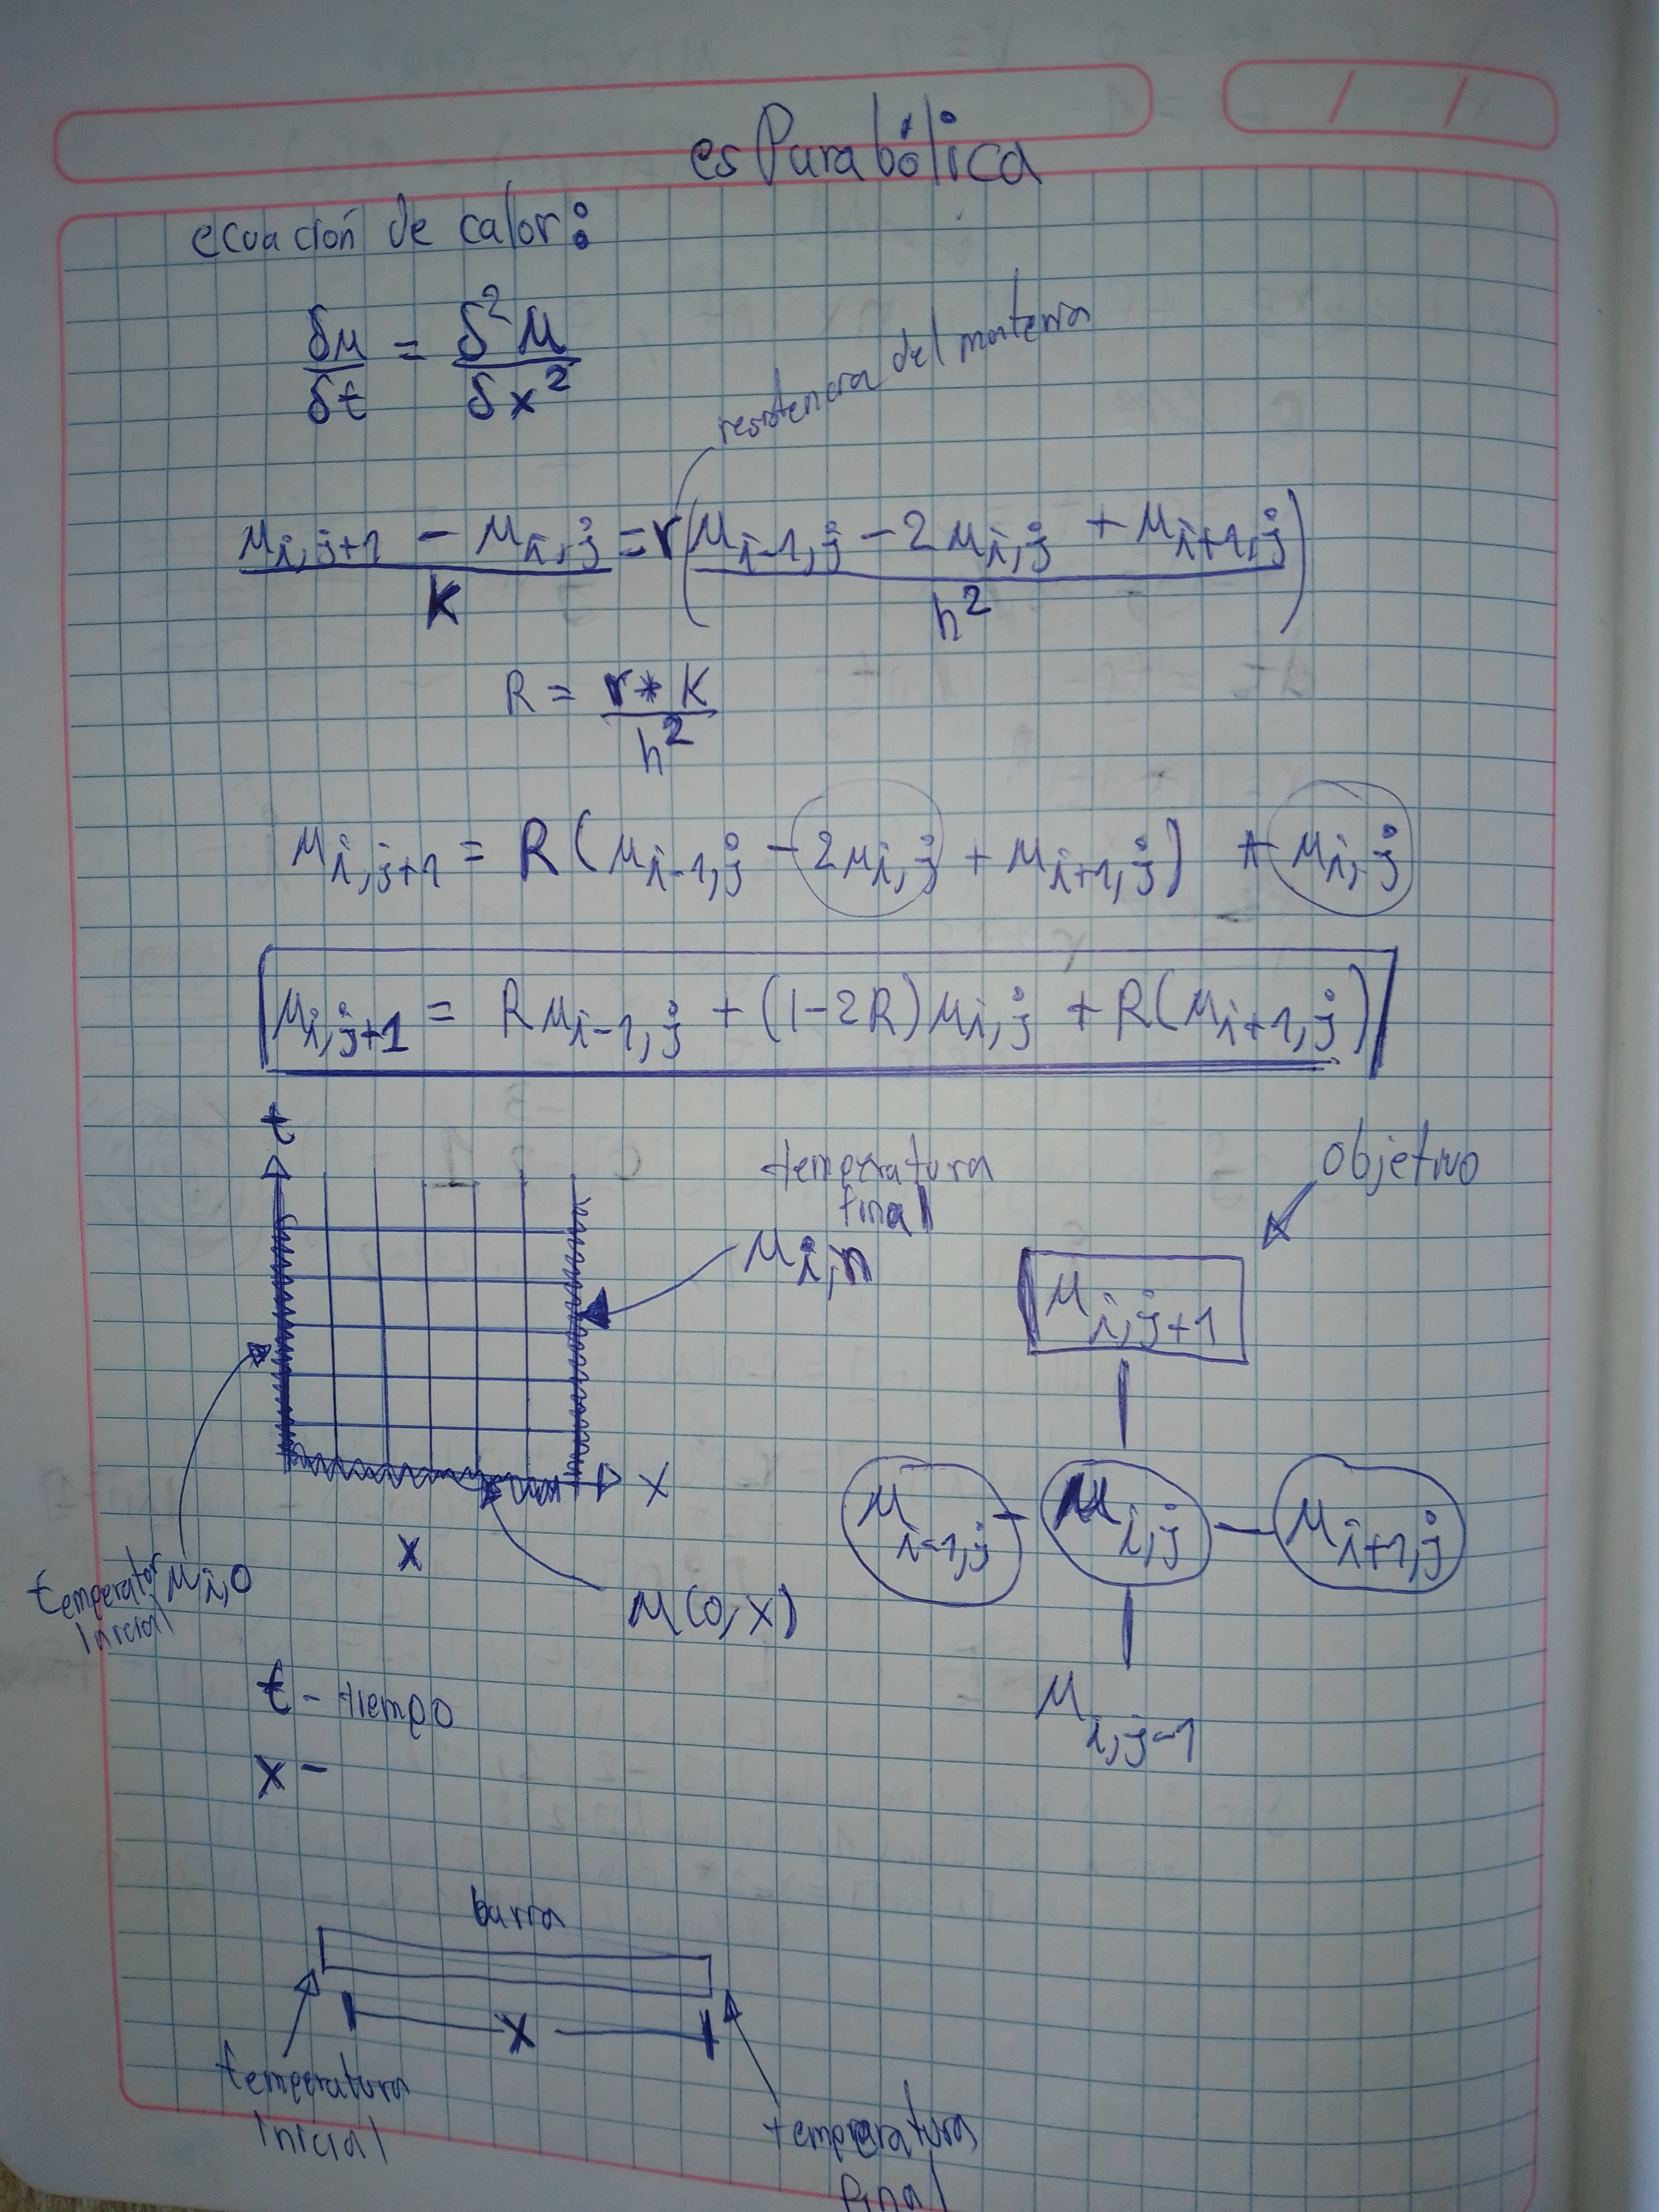
\includegraphics[width=0.7\textwidth]{analisis.jpg}
    \end{figure}

    \section{Programación}
    A continuación se presenta el codigo de implementación:
    \lstinputlisting[label=Archivo Ecuación de Calor]{heatEquation_v2.py}
    
    \subsection{Resultados}
    El resultado de la implementación anterior es:
    \begin{figure}[h]
        \centering
        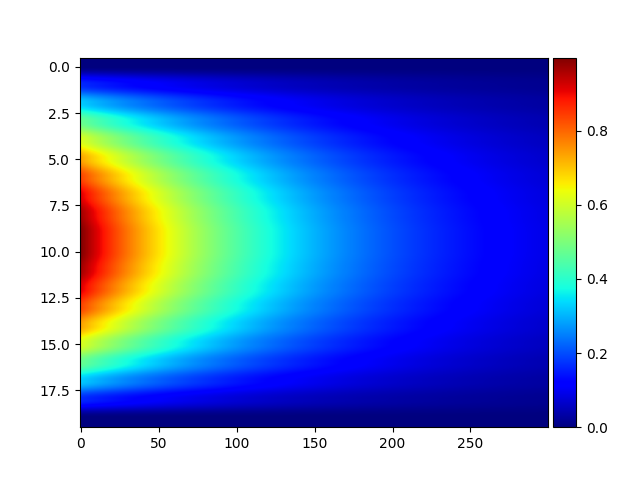
\includegraphics[width=\textwidth]{ejer1_graph.png}
        \caption{Función: \eq{sen(\pi x)}}
    \end{figure}
    \\\\\\
    En la anterior imagen tenemos dos gráficos, en el lago izquierdo tenemos
    el mapa de calor de la barra con respecto al tiempo, es decir la malla completa.
    Por el lado derecho, tenemos la grafica que son fragmentos de la malla cortada
    transversalmente, recogiendo fragmentos de la malla en diferentes partes del tiempo.

    La gráfica del lado derecho, nos muestra la propagación y la atenuación del cambio 
    de difusion de la temperatura desde el lado izquierdo de la barra hacia el lado derecho.

    Ambas gráficas muestran el comportamiento de la difusión de calor, la izquierda lo hace de manera continua, 
    mientras la otra lo hace en tiempos significativos.

    En la imagen izquierda podemos ver que en el segundo 0.9, el cambio de temperaturas
    ya no es tan brusco, a comparación del segundo 0.1.

    \section{Problema 2}
    Modifique el código anterior de manera que permitan resolver problemas 
    con condiciónes en la frontera de la 
    forma \eq{u(0,t) = g1(t) = 1} y \eq{u(a,t) = g2(t) = -1}.
\newpage
    \subsection{Programación}
    La implementación es la misma que el anterior problema, la función \emph{main()}
    es la que se cambia:
    \begin{lstlisting}[frame=single]
def main():
    f_test = lambda x: 0#no dan una funcion
    t_inicial = -1
    t_final = 1
    tiempo = 1 #segundos
    L = 1 #longitud
    gamma = 0.2 # resistencia del material
    heatEquation(0.001,f_test,t_inicial,t_final,t=tiempo,L=L,gamma=gamma)    
if __name__ == "__main__":
    main()
    \end{lstlisting}

    \subsection{Resultados}
    La gráfica resultante se muestra a continuación:

    \begin{figure}[h]
        \centering
        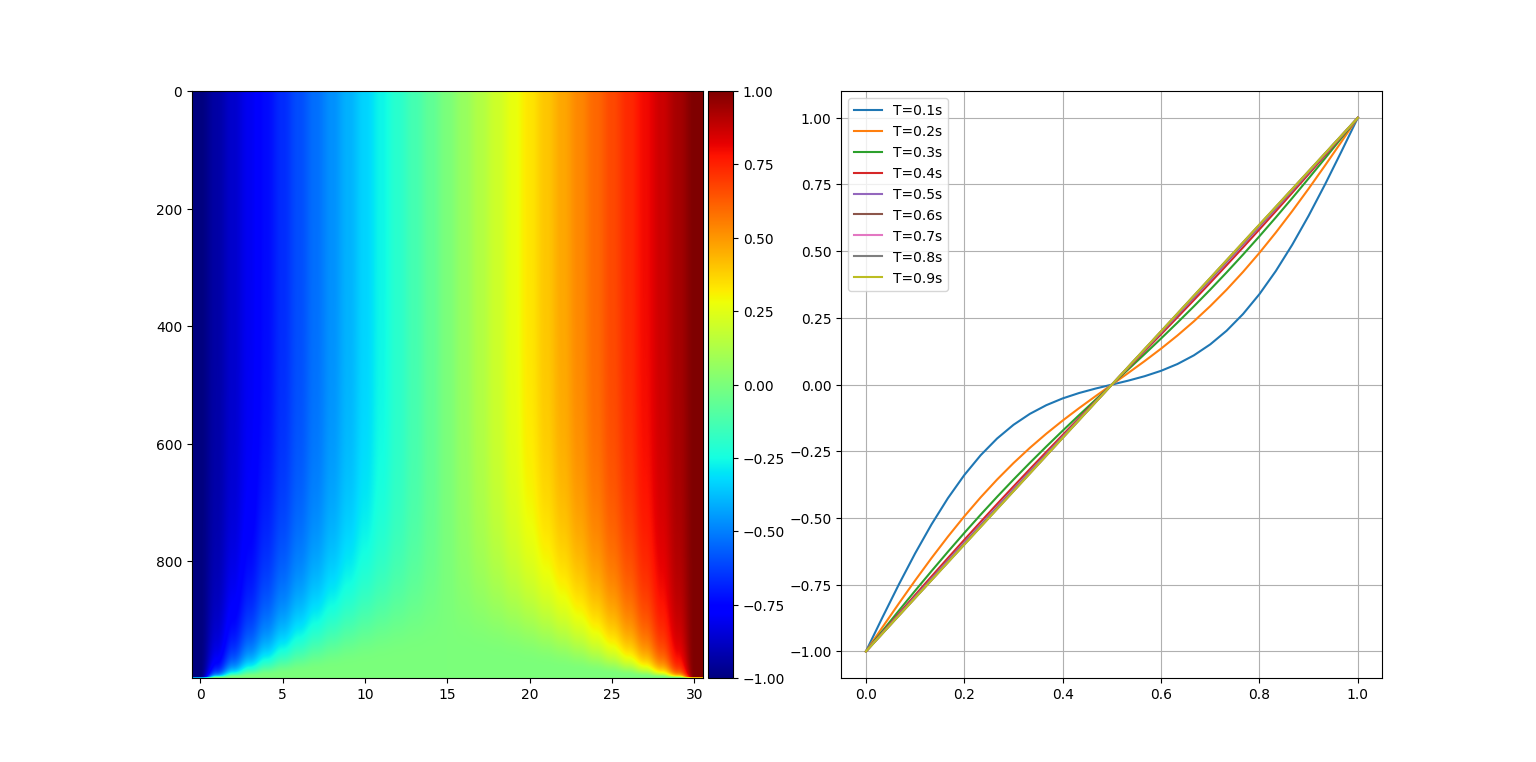
\includegraphics[width=\textwidth]{ejer2_graph.png}
        \caption{Ecuación de calor de -1 a 1}
    \end{figure}

    En la imagen anterior se muestra, como dos opuestos como temperatura en -1 de un 
    lado y una temperatura de 1 en el otro extremo, se propaga el lado con mayor temperatura
    hacia el de menor temperatura. Sin embargo luego de 1 segundo, la barra aún tiene 
    la misma temperatura en los dos extremos, esto se debe a que la temperatura en los extremos
    no varia debido a la especificación del algoritmo. Que expresamente indica que 
    una temperatura constante al inicio y al final de la barra en todo momento.
    \newpage    
    \section{Problema 3}
    Sea \eq{f(x) = sen(n\pi x) + sen(n + 1)\pi x}, busque valores de h y k para que
    tenga una solución estable y varié n para ver comportamiento diferentes
    en las condiciónes iniciales.
    \subsection{Programación}
    Como en el anterior ejercicio, lo único que cambio fue la función \emph{main()}:
\begin{lstlisting}[frame=single]
def main():
    n=2
    f_test = lambda x: m.sin(n*m.pi*x)+m.sin(n+1)*m.pi*x
    t_inicial = 0 #temperatura init
    t_final = 0 #temperatura fin
    tiempo = 1 # tiempo segundos
    L = 1 #longitud de barra
    gamma = 0.2 # resistencia del material
    heatEquation(0.001,f_test,t_inicial,t_final,t=tiempo,L=L,gamma=gamma)    
if __name__ == "__main__":
    main()
\end{lstlisting}

    \subsection{Resultados}
    En las siguientes imágenes se muestran la función evaluada en diferentes puntos de N:
    
    \begin{minipage}{\textwidth}
        Función con N=-1:\\
        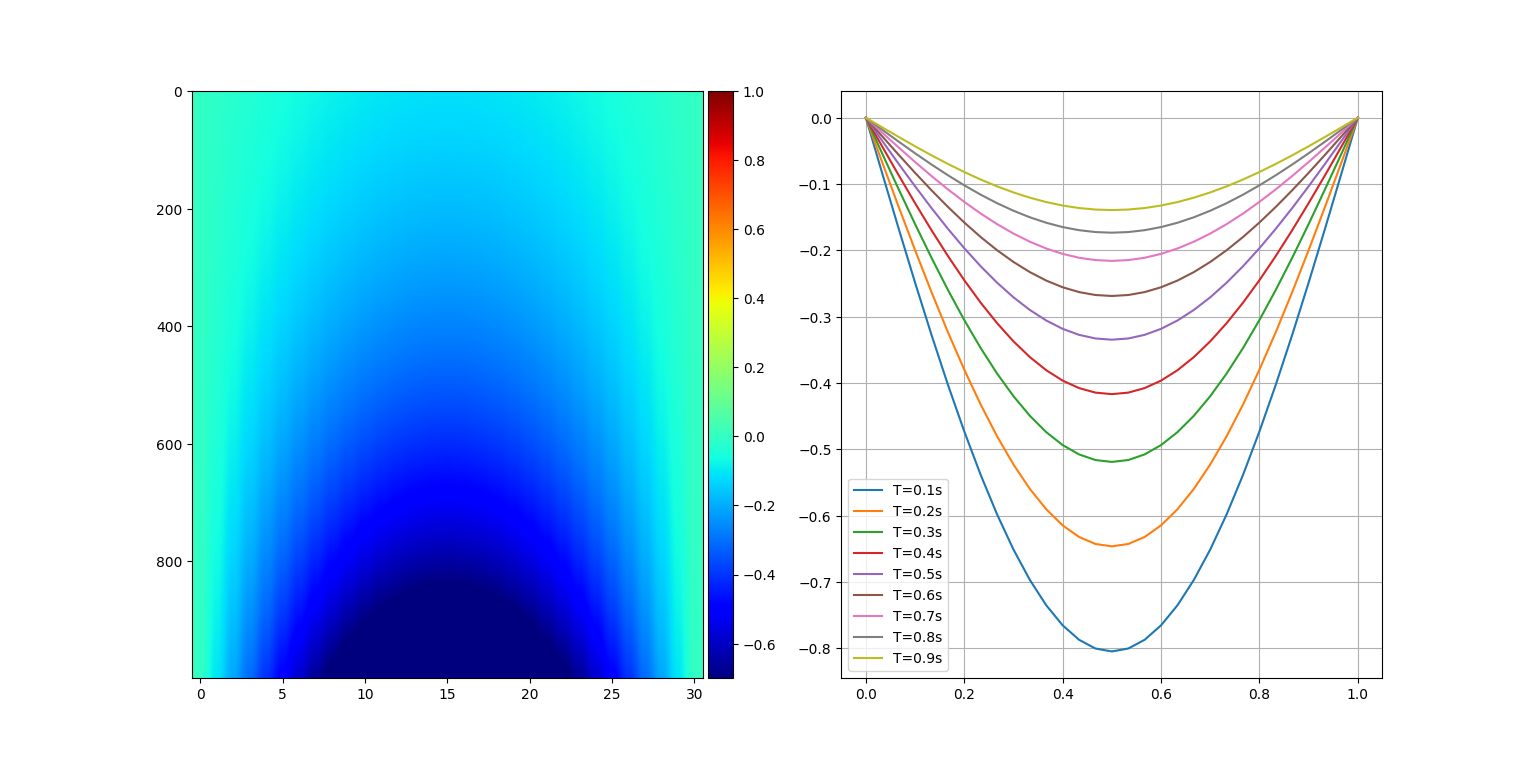
\includegraphics[width=\textwidth]{ejer3_4_graph.png}
    \end{minipage}

    \begin{table}[h]
        \centering
        \begin{tabular}{c}
            \begin{minipage}{\textwidth}
                Función con N=2:\\
                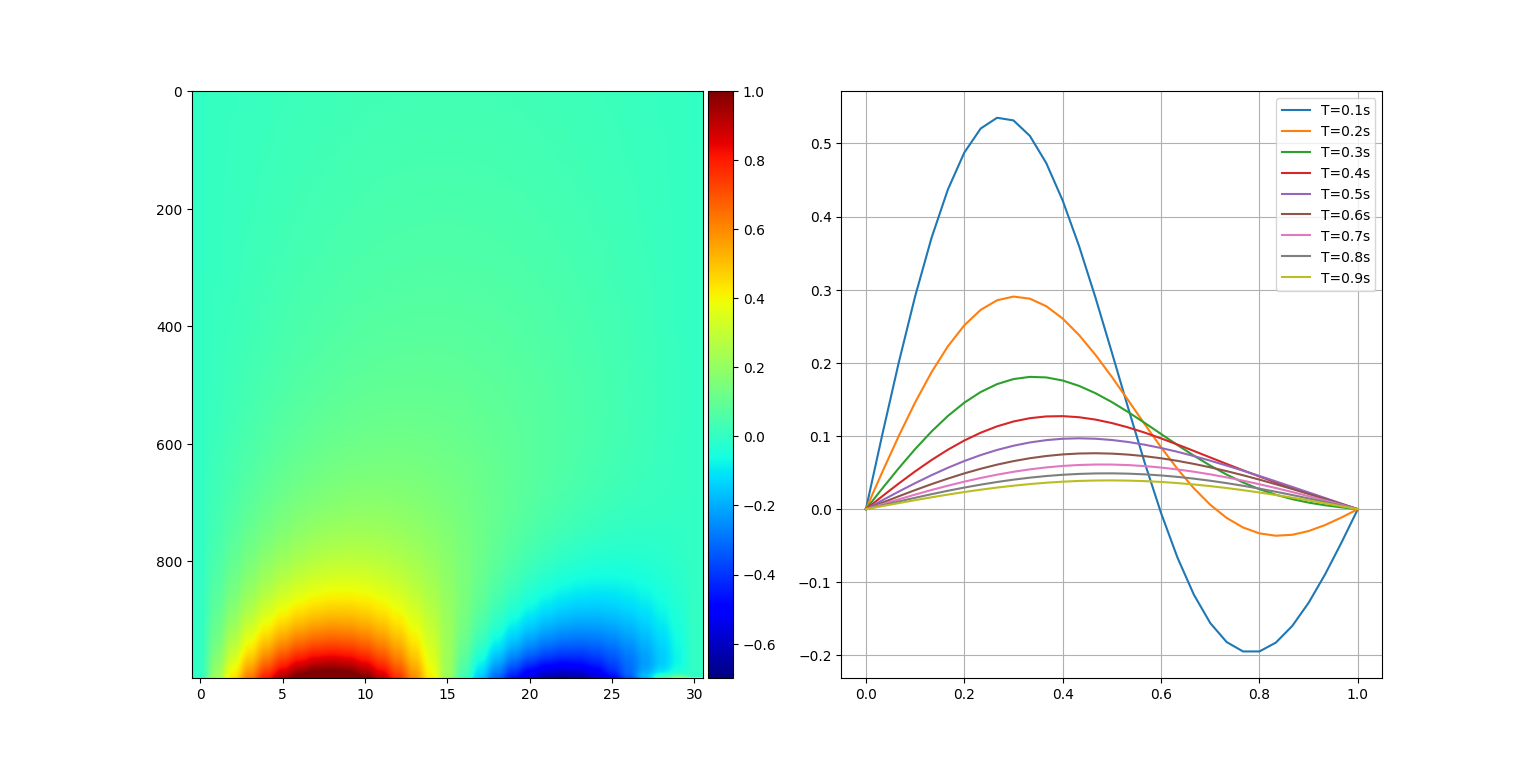
\includegraphics[width=\textwidth]{ejer3_graph.png}
            \end{minipage}\\
            \begin{minipage}{\textwidth}
                Función con N=1:\\
                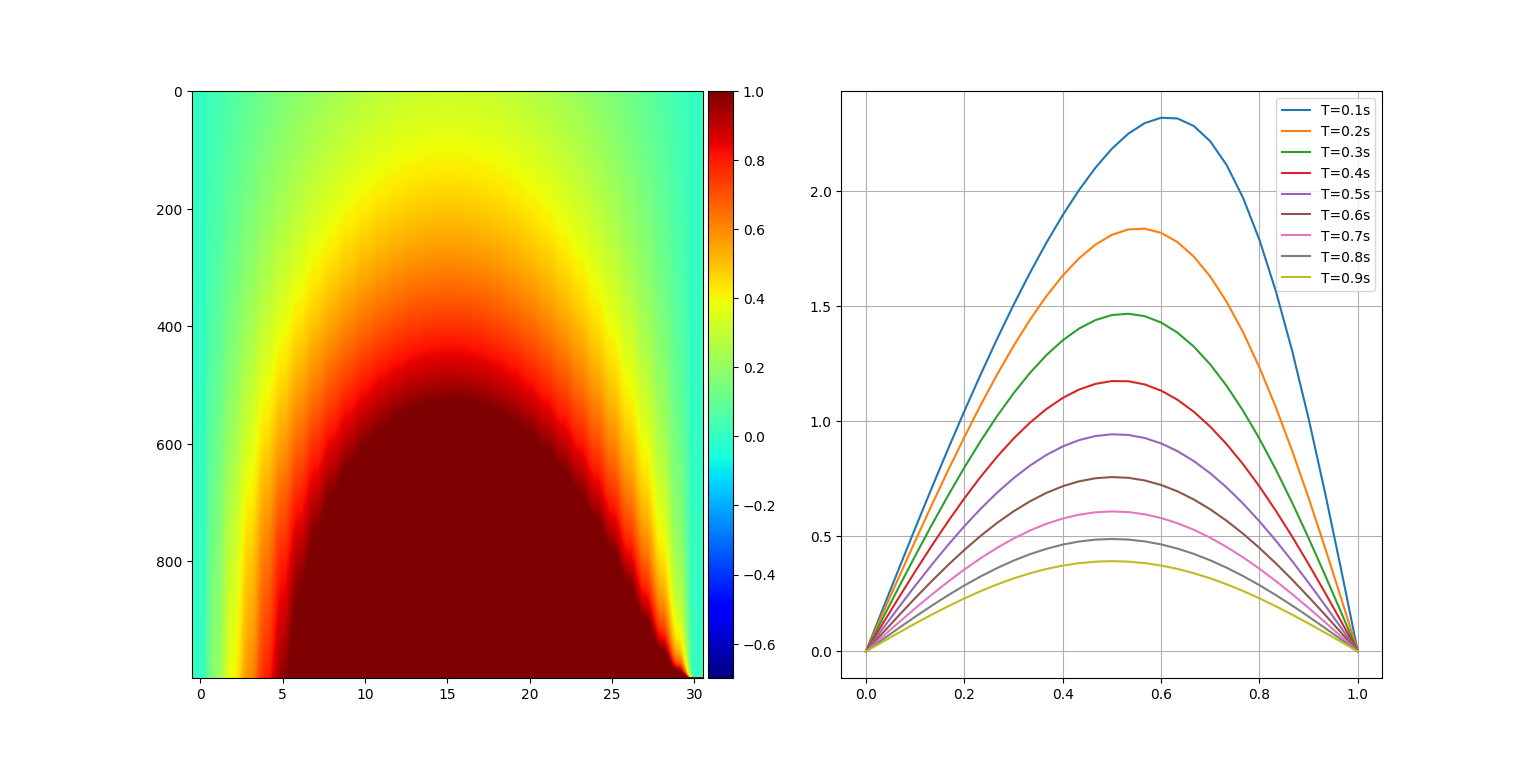
\includegraphics[width=\textwidth]{ejer3_1_graph.png}
            \end{minipage}
        \end{tabular}
    \end{table}    
    \begin{table}[h]
        \centering
        \begin{tabular}{c}
            \begin{minipage}{\textwidth}
                Función con N=0.5:\\
                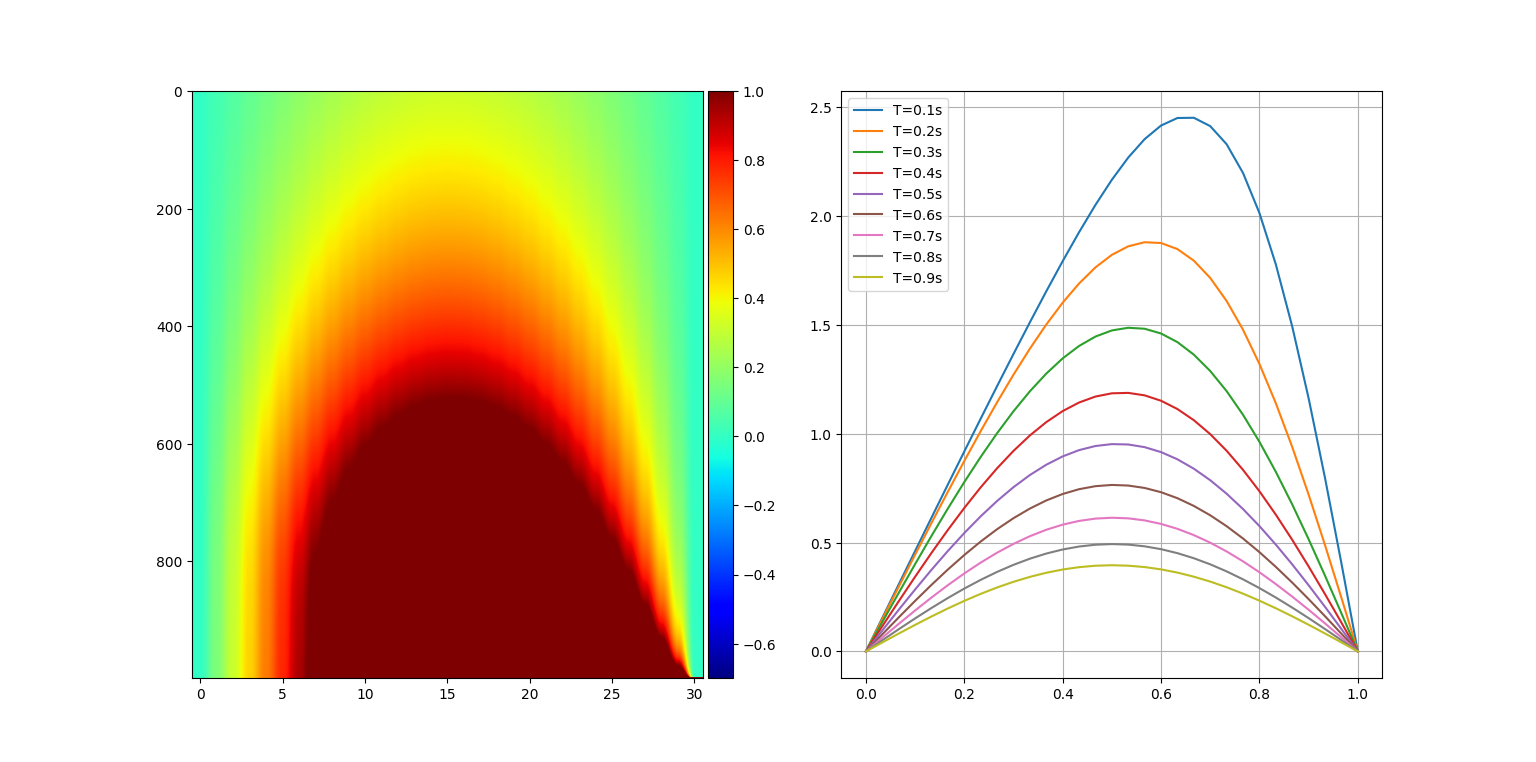
\includegraphics[width=\textwidth]{ejer3_2_graph.png}
            \end{minipage}\\
            \begin{minipage}{\textwidth}
                Función con N=0:\\
                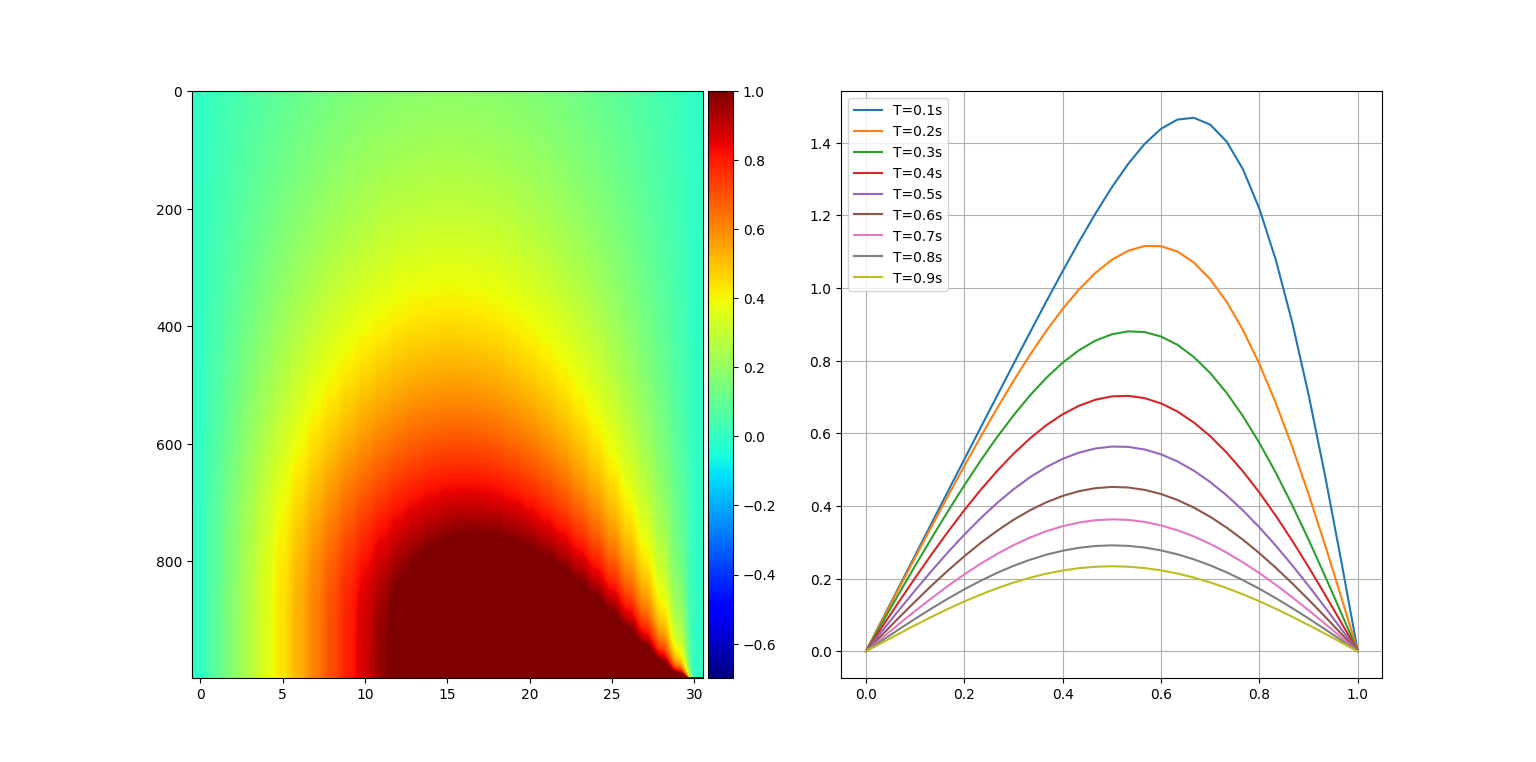
\includegraphics[width=\textwidth]{ejer3_3_graph.png}
            \end{minipage}
        \end{tabular}
    \end{table}
    

    \clearpage
    \section{Problema 4}
    Sea \eq{f(x) = 4 - \abs{4x-1} - \abs{4x-3}}, busque valores de h y k para tener
    una solución estable.
    \subsection{Programación}
    A igual que los ejercicios anteriores, se cambio el \emph{main()}:
    \begin{lstlisting}[frame=single]
def main():
    n=2
    f_test = lambda x: 4-abs(4*x-1)-abs(4*x-3)
    t_inicial = -1 #temperatura init
    t_final = -1 #temperatura fin
    tiempo = 0 # tiempo segundos
    L = 1 #longitud de barra
    gamma = 0.2 # resistencia del material
    heatEquation(0.001,f_test,t_inicial,t_final,t=tiempo,L=L,gamma=gamma)    
if __name__ == "__main__":
    main()
    \end{lstlisting}
    \subsection{Resultados}
    A continuación se muestra las gráficas de la función:
    \begin{figure}[h]
        \centering
        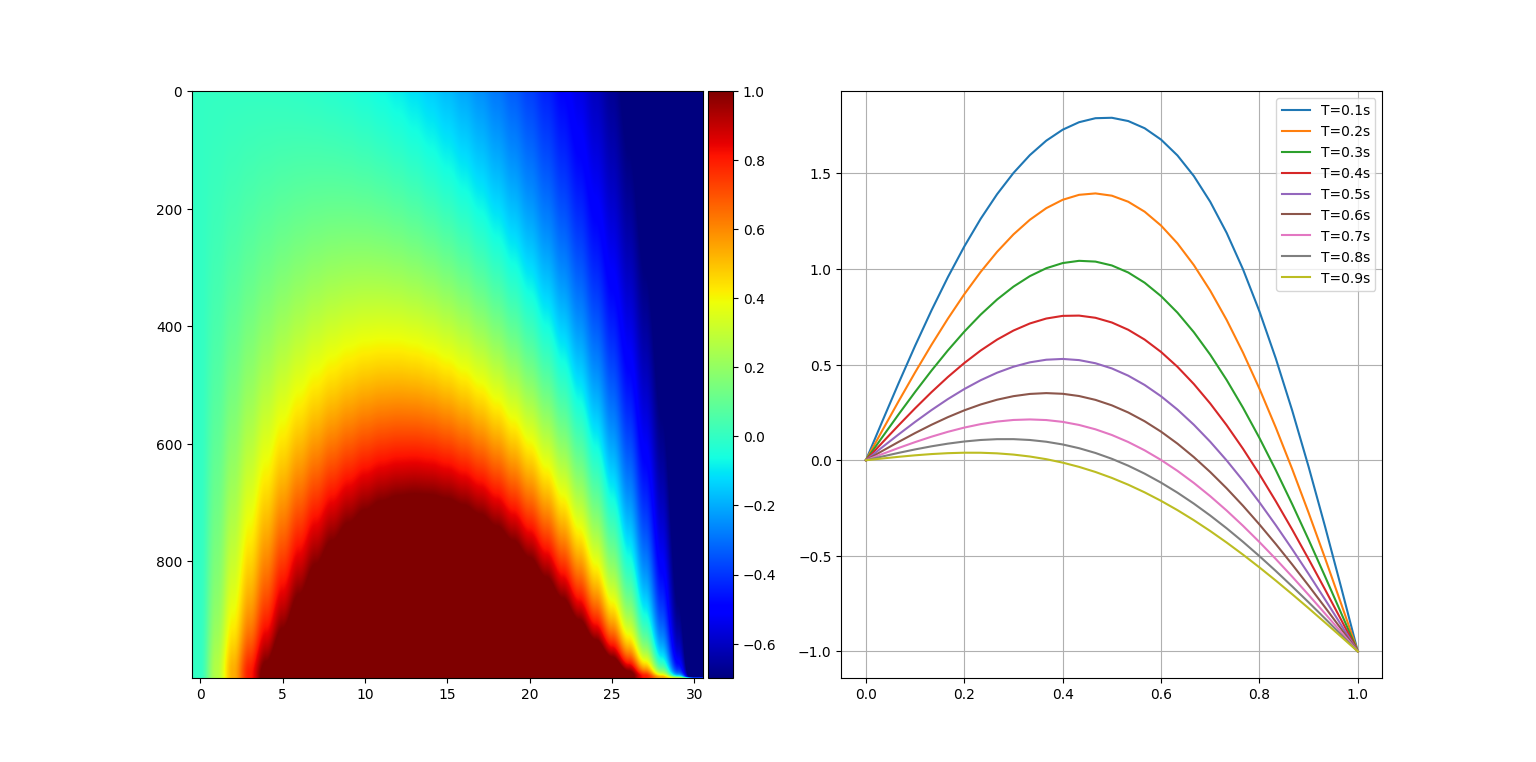
\includegraphics[width=\textwidth]{ejer4_graph.png}
        \caption{Función \eq{f(x) = 4 - \abs{4x-1} - \abs{4x-3}}}
    \end{figure}        

    En la anterior imagen se muestra que la temperatura del 
    lado izquierdo de la barra empieza en cero, y al otro lado extremo de la barra 
    se tiene una temperatura de -1. Y se puede apreciar como se atenua con respecto
    al tiempo el cambio de temperatura en la gráfica de la derecha en 1 segundo.

    \subsection{Análisis}
    La estabilidad sobre h y k es dada principalmente por que R, recoge 3 valores:
    \begin{equation}
        S = r\frac{k}{h^2}
    \end{equation}
    
    Donde \eq{S} es la resistencia del material, y \eq{k} es la diferencial con 
    respecto al tiempo, y \eq{h} con respecto a la longitud de la barra \eq{L}.

    La estabilidad siempre se da cuando \eq{S < 0.5}. 
    A continuación se muestra la imagen de la consola que imprime el valor S:
    \begin{figure}[h]
        \centering
        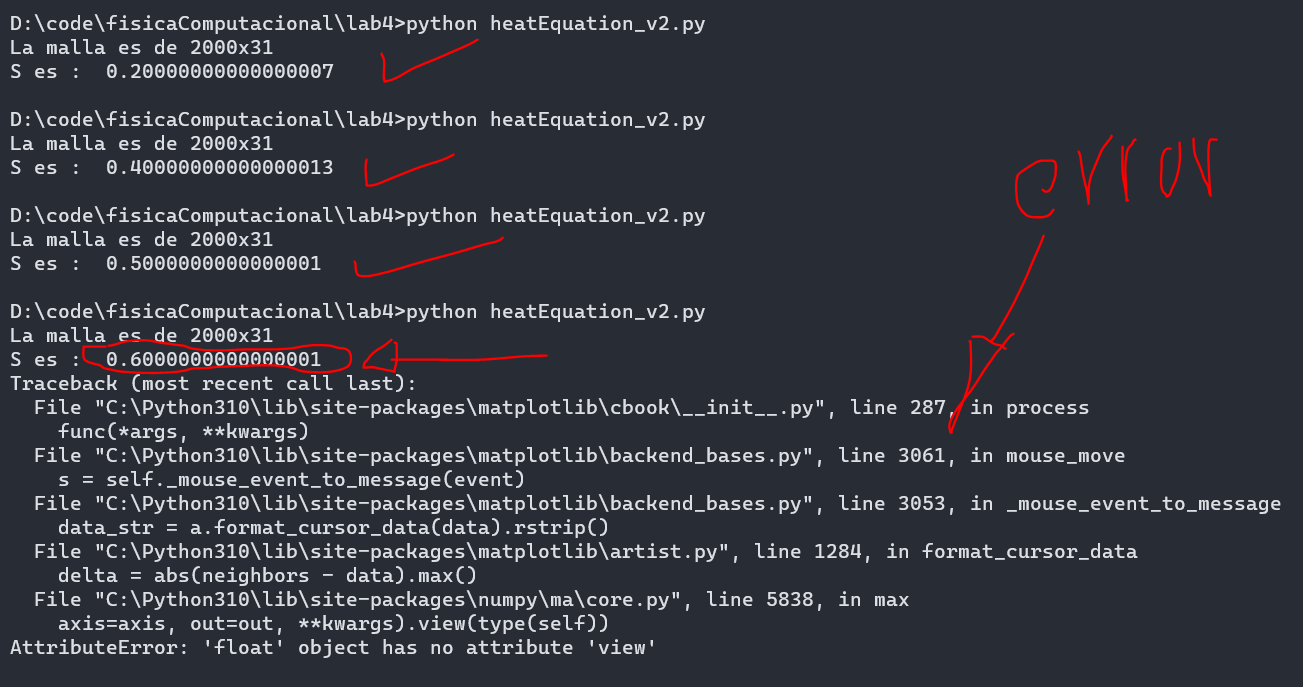
\includegraphics[width=\textwidth]{console4.PNG}
        \caption{Valor de S: \eq{S <= 0.5}}
    \end{figure}
    \clearpage    
    Y cuando el valor de \eq{S}, supera el valor de 0.5:
    \begin{figure}[h]
        \centering
        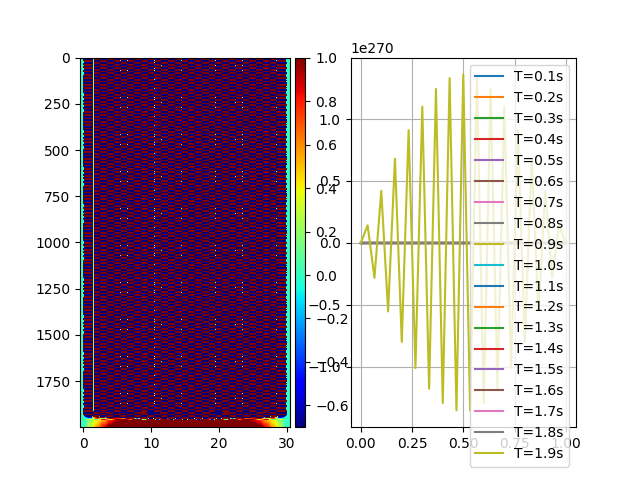
\includegraphics[width=\textwidth]{ejer4_1_graph.png}
        \caption{Problema 4 con \eq{S > 0.5}}
        \label{fig:erratic}
    \end{figure}

    Al igual que la imagen \ref{fig:erratic}, si se supera el umbral de 0.5.
    Todas las anteriores gráficas tienen el mismo comportamiento.

    Asi que por lo tanto si \eq{k} es demasiado grande y/o \eq{r} también.
    La función podria experimentar estos valores erráticos como en la gráfica \ref{fig:erratic}.

    \section{Conclusiones}
    La conclusion con respecto a la estabilidad cuando \eq{S < 0.5}, es una condición
    necesaria para la correcta interpretación de la gráfica.

    A esta restricción se le llama ``Courant Friedrich Lewy''.

    La cual especifica:
    \begin{equation}
        S = \gamma\frac{k}{h^2} \leq 0.5
    \end{equation}

    \end{document}
